\chapter{提案: ユーザレビューの分析および開発者支援ツール}
\label{chap:teian}

%ーーーーーーーーーーーーーーーーーーーーーーーーーーーー

\section{概要}
既存研究の多くはカテゴリやトピックを事前に定義した上で分類している. したがってレビューの特徴に応じてトピック, カテゴリの数や種類を変更することができないため, ``アプリの欠陥''や``開発者への要望''といった粒度の粗いクラスタリングしかすることができない. 
また, 既存研究では, トピック分類やキーワード抽出を実行した結果を示すところまでしか提案されていない. したがって, マイニングによって得られた結果を利用し, 開発者やユーザを支援するようなツールは提案されていない. 

したがって本論文では, レビューに含まれる開発に有用な情報 (アプリの欠陥やアプリに対する要望) を示す箇所 (以下 : キーフレーズ) のみを抽出し, キーフレーズを内容に応じてクラスタリングすることにより粒度の細かいクラスタリング手法を提案する. 
また, その結果をwebブラウザに表示することで, 開発者がレビューを閲覧, 分析しやすくするツールを提案する. 

\section{提案手法の流れ}
本研究で提案している手法やツールの流れを下記に示す. 

\begin{enumerate}
  \item Google PlayストアとTwitterに投稿されたレビュー及びツイートをスクレイピングして取得, 前処理
  \item キーフレーズを自動抽出
  \item 抽出したキーフレーズを利用しクラスタリング
  \item マイニングした結果をwebブラウザ上で可視化
\end{enumerate}

提案手法の流れを図\ref{fig:nagare}に示す. 

\begin{figure}[H]
  \centering
  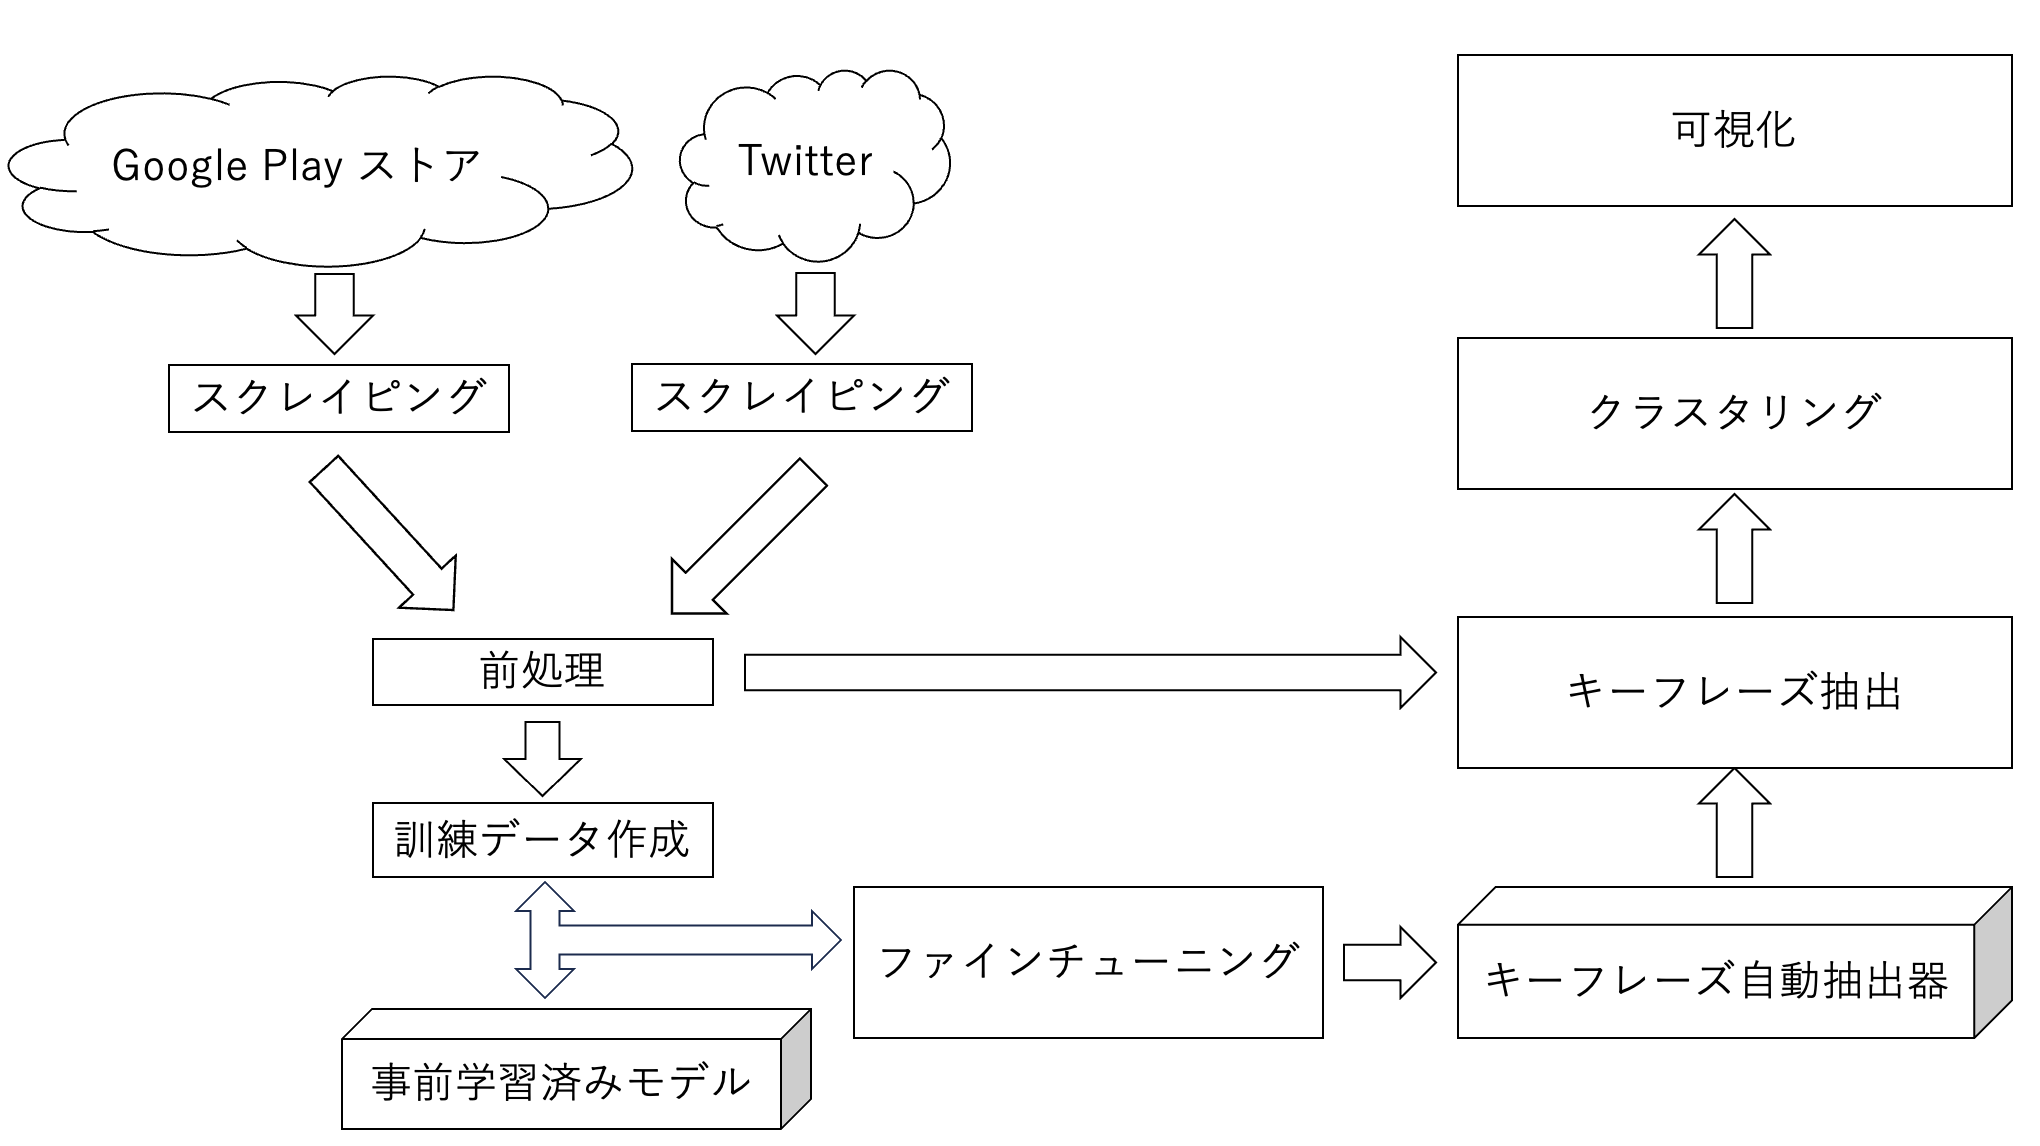
\includegraphics[scale=0.35]
    {contents/images/zisso.png}
  \caption{実装した提案手法の流れ\label{fig:nagare}}
\end{figure}

図\ref{fig:nagare}の各処理に関して, 実装の詳細を説明している節は次に示す通りである. 

\begin{itemize}
  \item Google PlayストアとTwitterからのスクレイピング: \ref{scraping}節
  \item スクレイピングされた情報の前処理: \ref{preprocessing}節
  \item 自動抽出: \ref{extraction}節
  \item クラスタリング: \ref{clustering}節
  \item 可視化: \ref{display}節
\end{itemize}

%ーーーーーーーーーーーーーーーーーーーーーーーーーーーー

\section{対象アプリとレビュー}
本研究では川面による先行研究\cite{kawatsura}のデータセットを使用するため対象アプリは先行研究のアプリに合わせている. 注意点として, BuzzVideoは2022年3月をもってサービスを終了しているため, 本研究で収集の対象となるアプリには含まれない. そのため, 本研究で新たに取得するレビューの対象となるアプリはBuzzVideo以外の12のアプリである. 
対象となっているアプリを表\ref{tb:taisyouapuri}に示す. 
\begin{table}[H]
  \small
  \caption{本研究の対象アプリ一覧}
  \label{tb:taisyouapuri}
  \begin{center}
  \begin{tabularx}{\linewidth}{l|l|X}
    \hline
    \mbox{アプリ名}\mbox{(一部略称)}&\mbox{Google Playストアの}\mbox{パッケージID}&\mbox{Twitterの}\mbox{検索キーワード}\\\hline\hline
    にゃんトーク&com.akvelon.meowtalk&にゃんトーク\\\hline
    スマートニュース&jp.gocro.smartnews.android&スマートニュース\\\hline
    PayPay&jp.ne.paypay.android.app&paypay\\\hline
    Coke ON&com.coke.cokeon&coke on\\\hline
    Google Fit&com.google.android.apps.fitness&google fit\\\hline
    Simeji&com.adamrocker.android.input.simeji&simeji\\\hline
    Lemon8&com.bd.nproject&lemon8\\\hline
    楽天ペイ&jp.co.rakuten.pay&楽天ペイ\\\hline
    majica&com.donki.majica&majica\\\hline
    LINE MUSIC&jp.linecorp.linemusic.android&line music\\\hline
    BuzzVideo&com.ss.android.article.topbuzzvideo&buzzvideo\\\hline
    ファミペイ&jp.co.family.familymart\verb|_|app&ファミペイ\\\hline
    CapCut&com.lemon.lvoverseas&capcut\\\hline
  \end{tabularx}\end{center}
\end{table}

%ーーーーーーーーーーーーーーーーーーーーーーーーーーーー

\section{事前準備}
本研究で対象としているアプリに関するGoogle PlayストアとTwitterのレビュー及びツイートをスクレイピングし, 分析対象となるデータセットを作成する. 本研究にて使用するデータセットは先行研究によって作成された13個のアプリレビューのデータセットに加え, 本研究で新たに収集した12個のアプリレビューのデータセットを使用する. 
対象アプリを先行研究に合わせた理由としては, 現在, Twitterの利用規約によりツイートの収集可能な数に制限がある影響で, 本研究だけでは十分な数のツイートが収集できなかったためである. Twitterのツイート取得数に関する制限は\ref{sec:x}で詳しく述べる. 
そして, スクレイピングしたデータから有用な箇所を自動抽出するために一般的な自然言語処理で行われる前処理を行う. 

%ーーーーーーーーーーーーーーーーーーーーーーーーーーーー

\section{有用な箇所の自動抽出}
\subsection{概要}
本研究における自動抽出の役割は次の2つである. 
\begin{itemize}
  \item 前処理された大量のレビュー (ツイート) から開発に有用な情報が記載されているレビュー (ツイート) のみを絞り込む
  \item レビュー (ツイート) からキーフレーズを抽出する
\end{itemize}
これによりアプリの欠陥やアプリに対する新たな機能の要望など開発に有用な情報のみが取得できる. 

\subsection{使用するモデル}
日本語のデータで事前学習済みの言語表現モデルである日本語BERTに対して質問応答形式のファインチューニングを行うことで自動抽出モデルを生成する. 
ファインチューニングのために, 元のレビュー文とアプリの欠陥や要望を尋ねる質問文, そして抽出したいキーフレーズを含めたデータセットを用意する. データセットの詳細は\ref{dataset}項で後述する. 
抽出対象となる元の文章の特徴をモデルに理解させるために質問文にその文章がGoogle PlayストアのレビューなのかTwitterのツイートなのかという``カテゴリー''の情報と``アプリ名''という2つの情報を加えることにより学習性能を上げる. 
図\ref{fig:fine-tuning}に質問応答形式によるファインチューニングのモデルを示す. 

\begin{figure}[H]
  \centering
  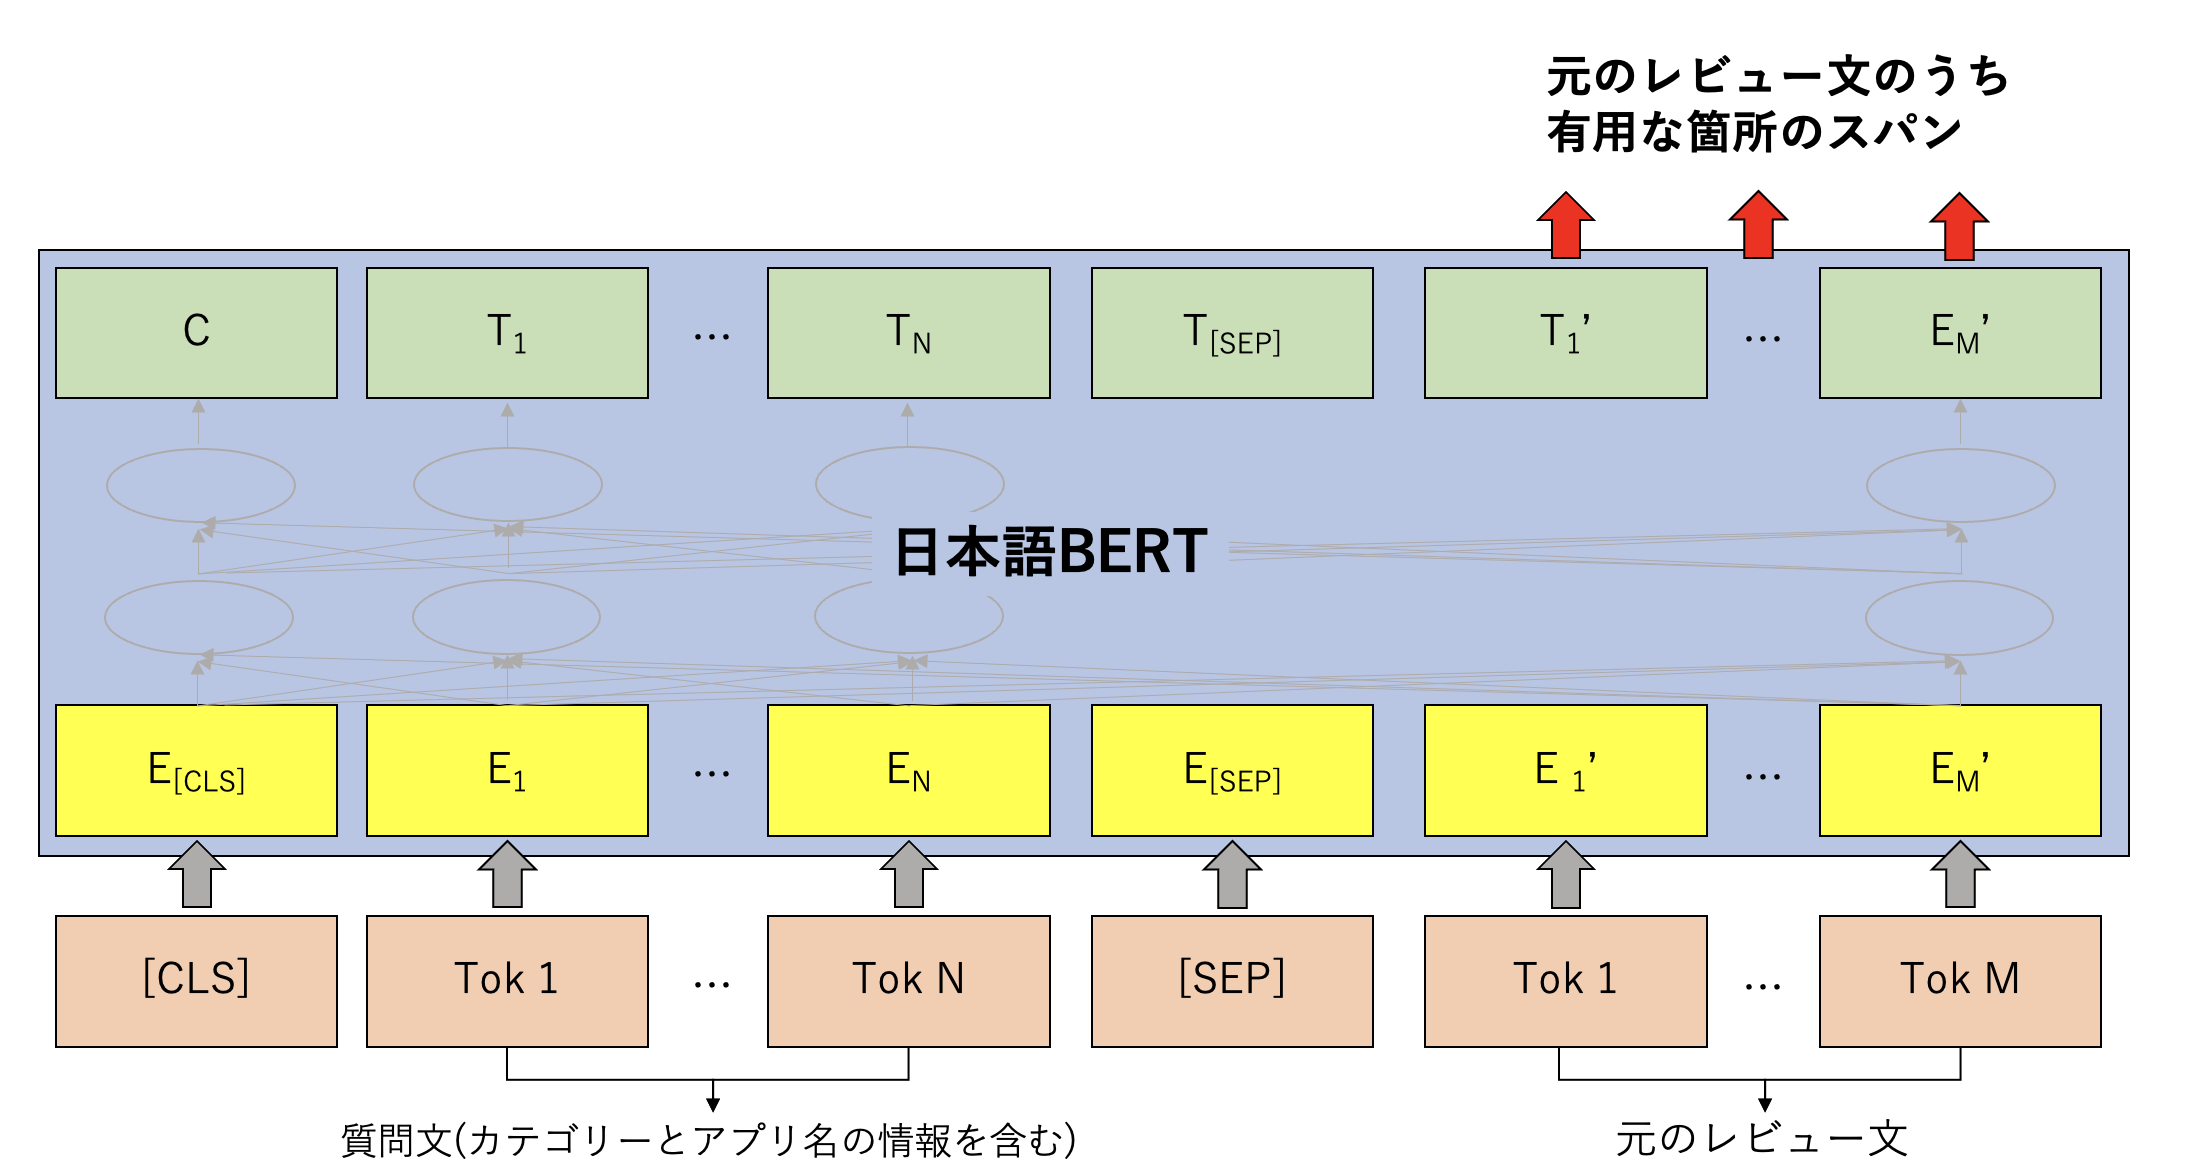
\includegraphics[scale=0.3]
    {contents/images/fine-tuning.png}
  \caption{ファインチューニング\label{fig:fine-tuning}}
\end{figure}

図\ref{fig:fine-tuning}に示したモデルでは, まず質問文と元のレビュー文をいくつかのトークンに分ける. この質問文には先述した通りカテゴリーとアプリ名の情報を含める. 
このトークンを用いて事前学習済みモデルをファインチューニングすることで, レビューに含まれるキーフレーズを抽出するためのモデルが生成される. 

図\ref{fig:answer}に質問文とその答えの例を示す. 質問文にアプリの欠陥やアプリに対する要望を尋ねる文章を与え, その答えとして抽出したキーフレーズを返すようにしている. 

\begin{figure}[H]
  \centering
  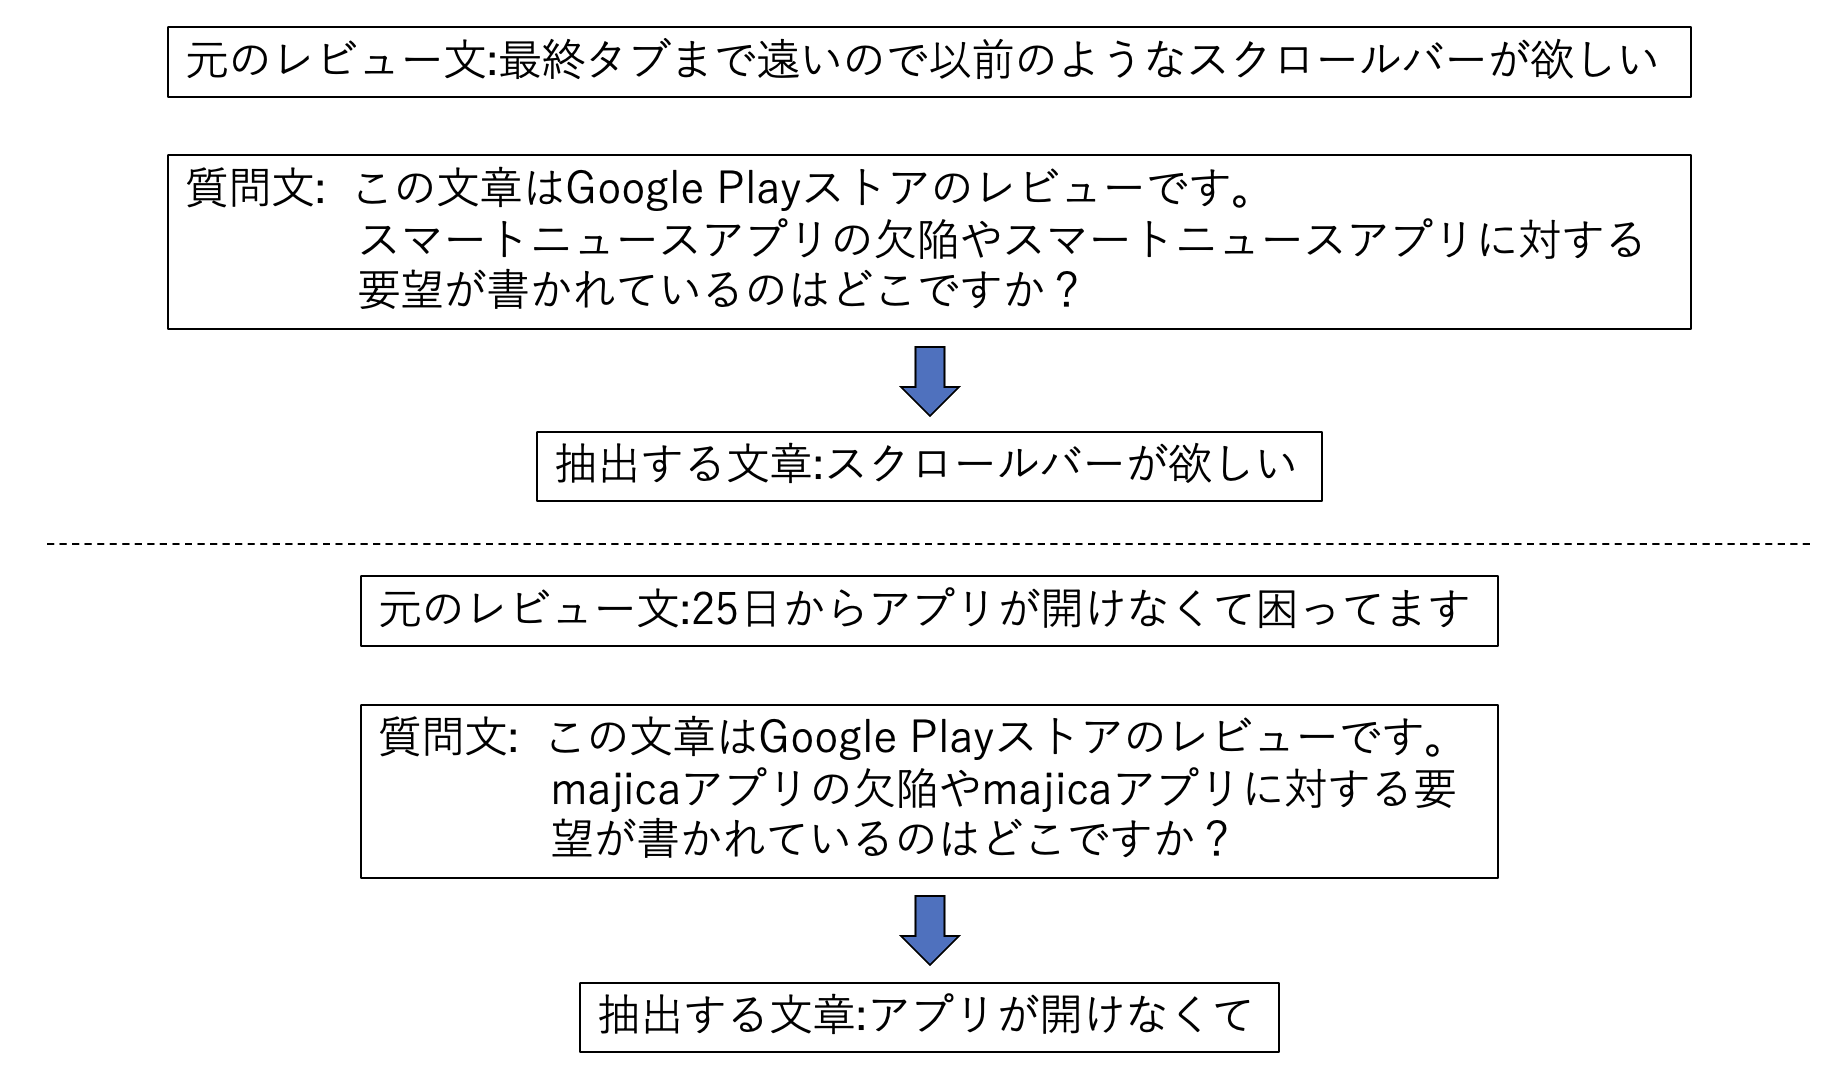
\includegraphics[scale=0.4]
       {contents/images/answer.png}
  \caption{キーフレーズの抽出例\label{fig:answer}}
\end{figure}

%ーーーーーーーーーーーーーーーーーーーーーーーーーーーー

\section{クラスタリング}
\subsection{概要}
本研究におけるクラスタリングの役割は次に示す2つである. 
\begin{itemize}
  \item 抽出された各キーフレーズを類似度に応じてクラスタリングする
  \item それぞれのクラスターにおける名称を決める
\end{itemize}

\subsection{クラスタリング手法}
抽出したキーフレーズのクラスタリングにはChinese Whispers\cite{chinese-whispers}を使用したグラフクラスタリング手法を提案する. グラフ作成のために抽出したキーフレーズをSentence-BERTの日本語モデルによってベクトルに変換する. Sentence-BERT\cite{sentence-bert}とは, 事前学習されたBERTモデルとSiamese Networkを使い, 高品質な文ベクトルを作る手法である. 
したがって本研究でのクラスタリング手法は下記の手順である. 
\begin{enumerate}
  \item Sentence-BERTの日本語モデルを用いて, 抽出した文章をベクトルに変換
  \item 重み付き無向グラフを構成し, 抽出したキーフレーズをノードとし, 2つの抽出した文章間のベクトル間のコサイン類似度スコアをノード間の重みとする. スコアがある閾値以上の場合, 2つのノード間にエッジを追加. この閾値は入力ハイパーパラメータであり, 抽出されたキーフレーズ間の意味的相関を測定するために使用される. 閾値が高いほどクラスターの結束力が高まる. 
  \item このグラフに対して, Chinese Whispers (CW) を実行し, 抽出したキーフレーズをクラスタリング. 
\end{enumerate}

図\ref{fig:clustering}にクラスタリングの概略図を示す. 丸で示されているのが抽出されたキーフレーズを表すノードであり, 点線がエッジである. このエッジは設定された閾値によって変化する. 
\begin{figure}[H]
  \centering
  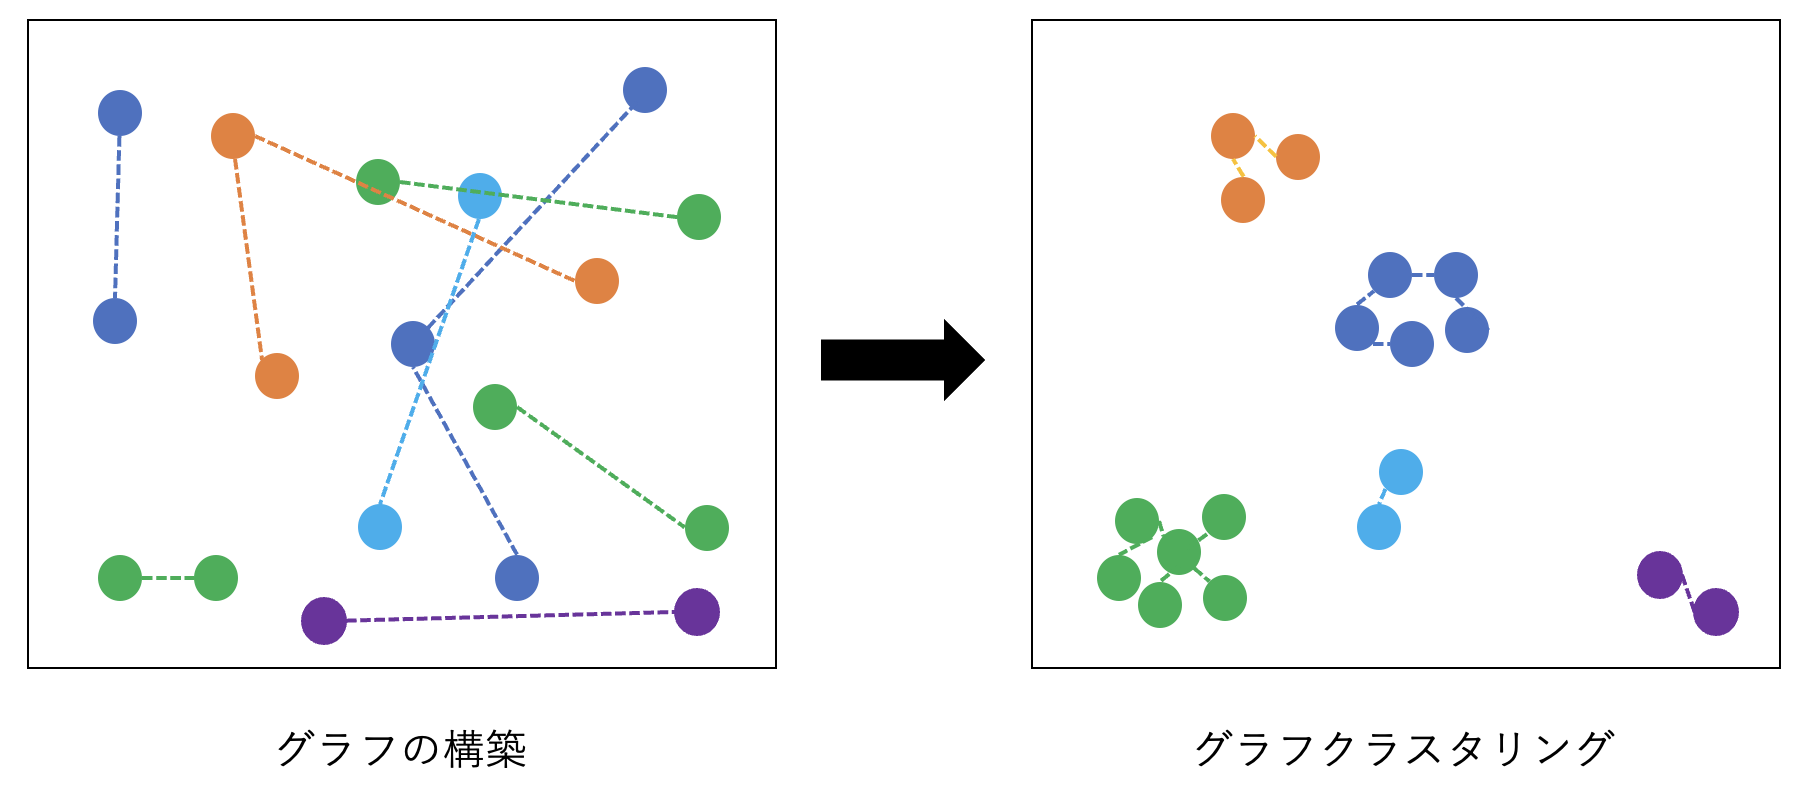
\includegraphics[scale=0.4]
       {contents/images/clustering.png}
  \caption{グラフクラスタリングの概略図\label{fig:clustering}}
\end{figure}

\subsection{各クラスターの名称}
クラスターを作成したら各クラスターの特徴を表す名称を決定する. 
この名称の決定にはKeyBERT\cite{keybert}を使用したキーワードの抽出によって実現する. KeyBERTとは, BERTの埋め込みを活用して, 文書に最も類似したキーワードを作成するキーワード抽出技法である. 
具体的な手順は次に示す通りである. 

\begin{enumerate}
  \item 文書レベルの表現を得るために, BERTを用いて文書埋め込みを抽出する
  \item N-gramの単語やフレーズについて単語埋め込みを抽出する
  \item コサイン類似度を用いて, 文書に最も類似する単語を見つける. 最も類似している単語は, 文書全体を最もよく表現する単語として特定される
\end{enumerate}

%ーーーーーーーーーーーーーーーーーーーーーーーーーーーー

\section{画面出力・可視化}
マイニングした結果を用いてwebブラウザで可視化を行う. クラスターごとにまとめて表示することで開発者が各レビューを確認しやすいようにする. 
開発者はアプリの修正やアップデートを行った後でユーザがどのようなレビューを挙げているかを特に確認したいと考えられる. したがって, 特定の機能や期間でのレビュー内容を確認できるよう, レビューが投稿された期間やキーワードで絞り込むことが可能な検索機能を実装した. 
そして, レビューの特徴を確認するために次に示す2つのグラフを作成した.
\begin{itemize}
  \item 日ごとのレビュー数を表す折れ線グラフ
  \item クラスターに含まれるレビュー数の上位10個を表す棒グラフ
\end{itemize}
この2つのグラフは検索結果に対応して変化するようになっている. 以上の機能を実装することにより, 開発者がレビューを理解, 分析しやすいように実装している. 